\chapter{Background studies} \label{stateofarts}
Before introducing the design and development of the prototype application, a fundamental base of knowledge has to be set. In this chapter, we give definitions about the most important terms and concepts used in VR. The context in which this project is set in is also explained briefly. Furthermore, we specify the most important technologies for the prototype and also point out where the limits of VR are. Finally, a measurement for the effectiveness of VR is presented.

\section{Context}
The prototype application focuses on the information technology diploma courses offered at the Nanyang Polytechnic. In the following, the environment of the school and the courses are described.

Nanyang Polytechnic (NYP) is a polytechnic located in Ang Mo Kio, Singapore. The school offers post-secondary education for students who successfully passed the GCE O-Level examination. This examination is mainly for students who have visited a secondary school. \cite{aboutOLevel} \\ 
Students are allowed to take courses either on a junior college, a technical institute or a polytechnic after passing the O-Level examination. In Singapore, a polytechnic offers students a more practical and industry based education than a junior college, which provides more widespreaded education. In general, students study three years at a polytechnic until they get their diploma. After getting a diploma, students can continue their education at a university or start to work in the industry. \cite{schoolSystem}
\subsection{Information technology courses at Nanyang Polytechnic}
NYP offers a wide range of courses in different fields. One of the fields is information technology (IT). In total, there are five courses. In the following, the courses will be introduced briefly: \cite{nypCourses}

\paragraph{Information Technology}
This course offers students a broad range of different fields in information technology. It focuses on interdisciplinary education. By finishing the course, students are prepared to work in different areas, most commonly in software engineering. During the first year, the fundamental topics of information technology are educated. The second year deepens the knowledge in application programming, database management, software engineering, algorithms and several other topics. The third year is for specialization. The students can choose between elective courses in the fields of artificial intelligence, enterprise cloud computing, geospatial and mobile innovation and cybersecurity. This course as well as all other IT courses at NYP offer one practical industry project and an internship in the third year.

\paragraph{Infocomm and Security}
This course covers topics in IT infrastructure, network engineering and security and the internet of things (IoT). Students learn how to program, but also how to secure applications in a connected environment and they learn about managing connected infrastructures. During the first year there are basic classes in programming and infocomm to get a grounded knowledge in information technology. The second year deepens the knowledge of network engineering, programming, and IT service management. There is a practical IoT project for students as well.
In the third year there are several elective courses in the areas of system and network security, enterprise infrastructure and infocomm solutions.

\paragraph{Cybersecurity and Digital Forensics}
The cybersecurity and digital forensic course focuses on IT security. This includes bewaring systems and data of unauthorized access as well as tracing criminals in case of a security incident. After graduating, students can work as security analysts, network penetration tester, security engineer and similar positions. During the first year, students learn fundamental IT skills. The second year offers classes in forensics, network security, operating systems, security standards and more. Students also complete an applications security and an infosecurity project.
The last year offers specialization in the topics cybersecurity  and cyber forensics. It is possible to choose cross-disciplinary classes from other IT courses.

\paragraph{Business Intelligence and Analytics}
The business intelligence and analytics course teaches analytics and interpretation of massive amounts of data. Therefore big data technologies as well as artificial intelligence is needed. After graduating, it is possible to work as a data or business analyst, a social media strategist or a digital marketing executive. During the first year students gain basic IT and business statistic knowledge. The second year offers classes in big data management, digital marketing, predictive modelling and similar topics. Students participate at a big data and business analytics project.
During the third year, students complete a data science project and choose between several elective classes.

\paragraph{Business and Financial Technology}
This course focuses on information technology in the financial and business sector. After getting a diploma, students can work as IT or financial consultants, financial application specialists or business and financial analysts. It is focused on connecting business and financial topics with information technology from the beginning. Therefore, in the first year students learn about economics, accounting and consumer banking as well as about basic programming skills. During the second year this knowledge is deepened through classes like software engineering or financial management. Besides the elective classes, the industry project and internship, students in their third year also collaborate in a fintech innovation project.

\subsection{What is virtual reality?}
According to \cite{Fuchs.2011} VR is a simulated virtual world, created with hardware and software. It provides a real time user interaction. Users feel the maximum amount of immersion when experiencing the computer generated world. The virtual world is mostly displayed through a head mounted display (HMD) as seen in figure \ref{fig:hmd}. This device splits the main scene into two different camera perspectives for each eye of the user. The two perspectives will then be merged into a three dimensional picture by the users brain. \\
\begin{figure}[h!]
  \includegraphics[width=70mm]{kapitel/eps/HMD-example.pdf}
  \centering
  \caption{Head mounted display by \cite{hmd1}}
  \label{fig:hmd}
\end{figure}
% by Maurizio Pesce -  \url{https://www.flickr.com/photos/pestoverde/17136177965}, CC BY 2.0, \url{https://commons.wikimedia.org/w/index.php?curid=39894108

The computation of the virtual world can either be done with a standalone desktop PC or with the HMD only, for example through a mobile phone which is wrapped inside the HMD.\\
Different than augmented reality (AR), VR provides a fully self-contained environment and does not interact with elements of the real world. AR on the other hand embeds virtual content into the real environment. Thereby, the borders between reality and simulation become blurry. \cite{Dorner.2013} \\AR is a closely related technology to VR, but this thesis will focus on VR applications only. In section \ref{dimensions-reality} we will differentiate VR and AR in more detail.\\
The usages of VR are very versatil. \cite{Linowes.2015} describes a variety of different areas in which VR can be used: Especially the gaming industry stands out for one of the first industries to develop VR applications and hardware devices. This is because most of the modern computer games take place in a computer generated, first person, 3d environment. To achieve a higher level of realism, it seems very promising to introduce VR in the gaming branche. Lately, non-gaming VR applications are getting more important. Design and architecture is a branch, where VR is used to visualise prototypes in a new way to customers. In education, VR applications are used to train learners in a nearly real environment but without the cost and danger of a real life exercise. Military training or disaster management are good showcases for the usage of VR in education. Another area, in which VR is used, is tourism. Through a VR application it is possible to visit a museum without actually travelling to the place. VR can give more immerse insights of a travelling destination and yet can be an instrument of marketing for the tourist destinations. For this work, the usage of VR in education  is very important.
\section{Virtual reality basic concepts}
\label{basic-concepts}
\cite{Sherman.2019} describe five core concepts for VR that are the key elements when it comes to design a virtual reality. In the following, these concepts are explained:
\paragraph{Participants} A participant is a user of a VR application, who is actually wearing the HMD and experiencing the virtual world. Every participant has a different perception of the application. Therefore every experience is a unique experience due to the cultural background of the participants, their age, their expectations and their knowledge in technology. Therefore, it is a challenge for developers of VR applications to create a virtual world that various users can identify with. The role of the participants is described as the most important role, because all the experience is happening in their imagination. Developers or creators are only capable of creating the framework around the experience.
\paragraph{Creators} Creators or developers design and implement a VR application for participants. As mentioned, the developers are not able to create the experience of the users. The core aim of their work is to develop the application, which is a collection of programming scripts, concept designs and data. The experience is created together with the participants. Later in this thesis we will give an insight in developing a VR application from a creator's perspective, whilst chapter \ref{testing} will dive into the different experiences of participants using the VR application.
\paragraph{Virtual world} In general, the term "virtual world" is defined as the content of a virtual reality application.  The virtual world is the skeleton of the virtual experience. Precisely, it is a description of the objects inside the virtual space. Everything which the user can see, hear and interact within the VR application belongs to the virtual world. The experience of a participant is influenced by the design of the virtual world space.

\paragraph{Immersion} Immersion in general describes how deeply users connect with a virtual world. Users experience something through a medium that they would not be able to experience without it. They see actions and things from a different point of view and can connect with it in some way. The deeper users can connect to the virtual environment and the objects inside it, the more immerse is the VR experience. In chapter \ref{immersion} the term immersion will be explained in more detail.

\paragraph{Interaction} Most commonly, interaction means manipulation of a computer generated world. However, interaction can also happen in a non artificial environment. An example for this are interactive novels or text based computer games. In this kind of media, computer graphics are not required and yet provide a form of user interaction. When it comes to VR, interaction also means relocating a viewport inside a virtual world. Participants can move physically in the virtual environment. Another form of interaction is the collaborative interaction. In some VR applications it is not only possible to interact with the virtual world but also to share the space with other participants and interact with them. This can happen in a virtual or physical way.
\subsection{Different dimensions of reality}
\label{dimensions-reality}
Besides VR there are other technologies which serve the purpose of creating virtual worlds for the user. They differ in the extend of intervention with reality. \cite{Tham.2018} show a spectrum of different types of technologies and their dimension of reality. A visual representation of this spectrum is displayed in \ref{fig:spectrum}.\\
\begin{figure}[h!]
  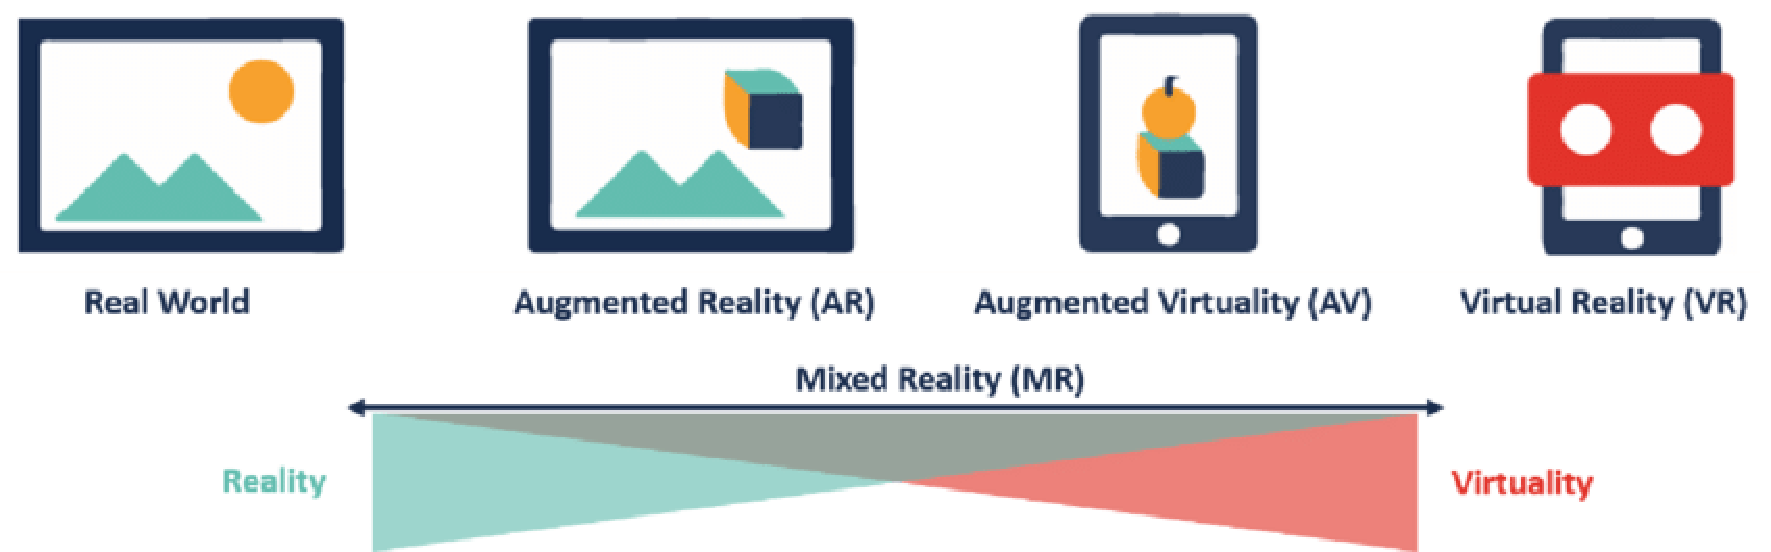
\includegraphics[width=14cm]{kapitel/eps/spectrum-of-reality.pdf}
  \centering
  \caption{Graphical representation of the dimensions of reality by 	  \cite{Lovreglio.2018}}
  \label{fig:spectrum}
\end{figure}

The reality describes the real world and uses non digital devices for interaction, such as a steering wheel for driving a car. As mentioned in the indroduction, AR is a related technology to VR. In the spectrum of \cite{Tham.2018} AR covers the second level of reality dimensions. It describes computer generated elements which are embedded into the reality. A famous example for an AR application is the game PokemonGo \footnote{\label{foot:1} for further information see: \url{https://www.pokemongo.com/en-gb/}}, in which players search, based on a phone's camera and location services, in the real environment for computer generated items. The next level of reality is the augmented virtuality. This term describes a virtual environment, in which users can interact through analogue methods. An example for this is a video chat room where the participants are present in a virtual room but communicate through analogue methods. As seen in figure \ref{fig:spectrum}, augmented reality and augmented virtuality can be summed up with the term "mixed reality" which describes the interaction between real life elements and the virtual environment. Finally, in the last stage there is VR in which a user is fully surrounded by a computer generated environment. This environment is most likely a reproduction of a real-life environment. The user is not only surrounded by an artificial reality but can also interact with it. It might happen that the user actually feels present in the virtual reality. In the following, this phenomenon will be explained in more detail.

\subsection{Immersion and storytelling}\label{immersion}
The term immersion is already introduced shortly in section \ref{basic-concepts}.
It is an important measurement for this work. An immerse experience for this VR application means that students can dive into the IT job roles and get a real insight from a first person's view. It is expected that the higher the grade of immersion is, the better participants can understand the IT job roles.\\
When talking about immersion, it is important to distinguish between  mental and physical immersion. Mental immersion describes the state in which the participant feels deeply emotionally connected to the virtual world. Physical immersion on the other hand means that the user's physical interactions are transferred into the virtual environment with the use of technology. The movements should feel as natural as possible to the user. When talking about immersion in books, films or related media, it is often only referred to mental immersion because these types of media are not able to provide the technology for interacting with their environments. VR on the other hand can create immersion through a physical way as well. That is why VR can provide a higher grade of immersion than other media. \cite{Tham.2018}\\
Another term closely related to immersion is presence. Presence in the context of VR describes the subjective feeling of actually existing in the virtual world. The feeling of presence is a mix between mental and physical immersion. The more presence users feel, the more they accept the virtual world as the reality. To gain a sense of presence, the participant's movements in the reality should match with the movements of the virtual world.
With a higher grade of presence, participants act more natural in a virutal environment, similar to their behaviour in a real environment. Through this, their task performance increases. This is a reason why presence is an important factor when it comes to developing VR applications, especially in the field of education and learning. \cite{Slater.1997}
\newpage
Now that the terms immersion and presence are explained, the question is now, how to design the story of a VR application in order to gain a maximum immersion. Storytelling is one of the most important elements for mental immersion in a virtual experience. Especially mental immersion can be influenced by the storyline, while physical immersion can be increased through hardware tools \cite{Tham.2018}. Since the access to hardware tools is limited by the school in this project, we rely on a good storytelling to increase the immersion of the VR prototype. \\
Storytelling in general is the art of telling a narrative to the user in a way that the user is not only consumer but actually feels immersed with the story \cite{Louden.2018}. Designing a storyline in VR opens a lot of possibilities in engaging the participant with the story. When it comes to storytelling in VR, the following things should be considered:\\
One thing to bear in mind is, that space and environment in a VR application are more important than in other media, like books or films. The creator designs a world in a 360 degree view, so there is a lot more space to show. The storyline not only happens in front of the users, but can be all around them. Because the user is able to walk independently in the virtual world, it is very important to softly guide users into a certain direction when necessary for the storyline. The guidance should not be conspicuous, but should attract  users' curiosity. This can be achieved through light and sound effects or movements. Another aspect to consider is not to overwhelm  users with complex tasks. This could prevent the user in experiencing an immersed virtual world because their full attention would lie on completing the tasks. \cite{Keane.2018}
\subsection{Interaction: Selection, manipulation and navigation}
\label{interaction-state-of-art}
Users of a VR application need to interact with the environment in order to increase immersion. Several challenges occur when dealing with interaction in VR. First of all, there is a three dimensional space which has to be covered. Secondly, when users are wearing the HMDs, they cannot see the controllers they are using in the real world. This means that every hardware controlling device should be mapped into the virtual world. In this chapter we describe some typical interactions and their common solutions in VR. It is a basic overview of interaction methods, which are considered to be used in the prototype VR application. The final method, which suits the best for the prototype, is discussed in chapter \ref{design}.\\
Basically, there are two different types of interaction in VR: Modifying the virtual world and moving in the virtual world. When modifying the virtual world, the user should be able to select and manipulate objects. Manipulating includes moving, scaling, changing of look (colour, texture) and orientation of an object in the virtual world. When walking around in the virtual world, the user should be able to move freely and make their own decisions in navigation. \cite{Dorner.2013}\\
A challenge when finding solutions to the described interaction problems is, that there do not exist standard solutions, like we have in a screen based 2D context for example. Nevertheless, There are some best practices on how to implement the described requirements in VR. \cite{Dorner.2013} describe some of the most common interaction techniques. \\For this section, we explain the techniques, which we most likely consider to use in the prototype of this work: gaze selection, ray-casting, Go-Go, HOMER and world in miniature.
\begin{figure}[]
	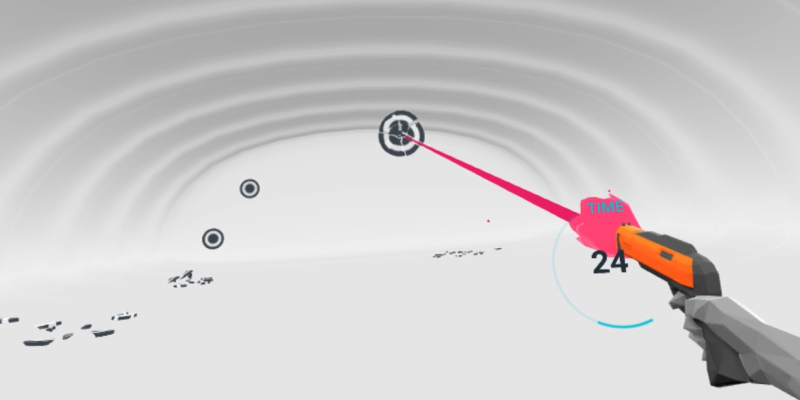
\includegraphics[width=14cm]{kapitel/ray-casting.jpg}
	\centering
	\caption{Selection of targets through ray-casting in the Oculus sample scenes \cite{Goldstone.2015}}
	\label{fig:ray-casting}
\end{figure}

A very straightforward method in selection could be the \textbf{gaze selection}. The user can select objects by looking at it. This is a very simple method and works without hardware controllers for user input. An analogy in 2D interfaces would be the selection via mouse over. However, this technique does not work well in VR. The problem is, that users accidentally select objects every time they look around. A simple and natural exploring of the virtual world would be interrupted by object selection.\\
\textbf{Ray-casting} works with a virtual ray coming from the users' hand, which can be seen in figure \ref{fig:ray-casting}. Therefore, a controller or a hand tracking hardware is needed which movements are mapped into the virtual world. Every object which collides with the ray is a possible candidate for selection. Most of the time, the object nearest to the user will be selected. ray-casting is an important method in object selection, because it is very straightforward and meets with the expectations of users. Nevertheless, this method becomes inaccurate when dealing with large distances, because the movements of the hand has to be more accurate the longer the distance gets. \\
The next method, the \textbf{Go-Go technique}, overcomes this problem. A virtual arm, mapped with the user's hand movements is displayed in the virtual world just as done with the ray-casting method. The difference of the Go-Go- technique is that the virtual arm can be lengthened, if selectable objects are out of range. When the virtual arm is lengthened, the user's hand movements are mapped into a smaller range than if the virtual arm is in a normal position. This mapping is not linear and overcomes the problem of inaccuracy when selecting objects too far away. The technique can be used for relocating objects, because the user does not have to walk on the same time. However, only objects which are in viewing range can be selected or manipulated with this technique. Some objects could be hidden by other obstacles and cannot be selected. Also, objects in far distance appear very small, which makes manipulation difficult.\\
The \textbf{HOMER technique} deals with manipulation of objects in the distance. The abbreviations stands for Hand-Centered Object Manipulation Ray-casting. As the names says, it uses techniques of ray casting for selection. To make a manipulation easier, the object moves to the users hand after selection. The user can now perform their desired manipulation. After the manipulation is finished, the objects teleport back to their original position. This technique still has the problem of selecting objects which are not in the user's viewing range.\\
\begin{figure}[h!]
  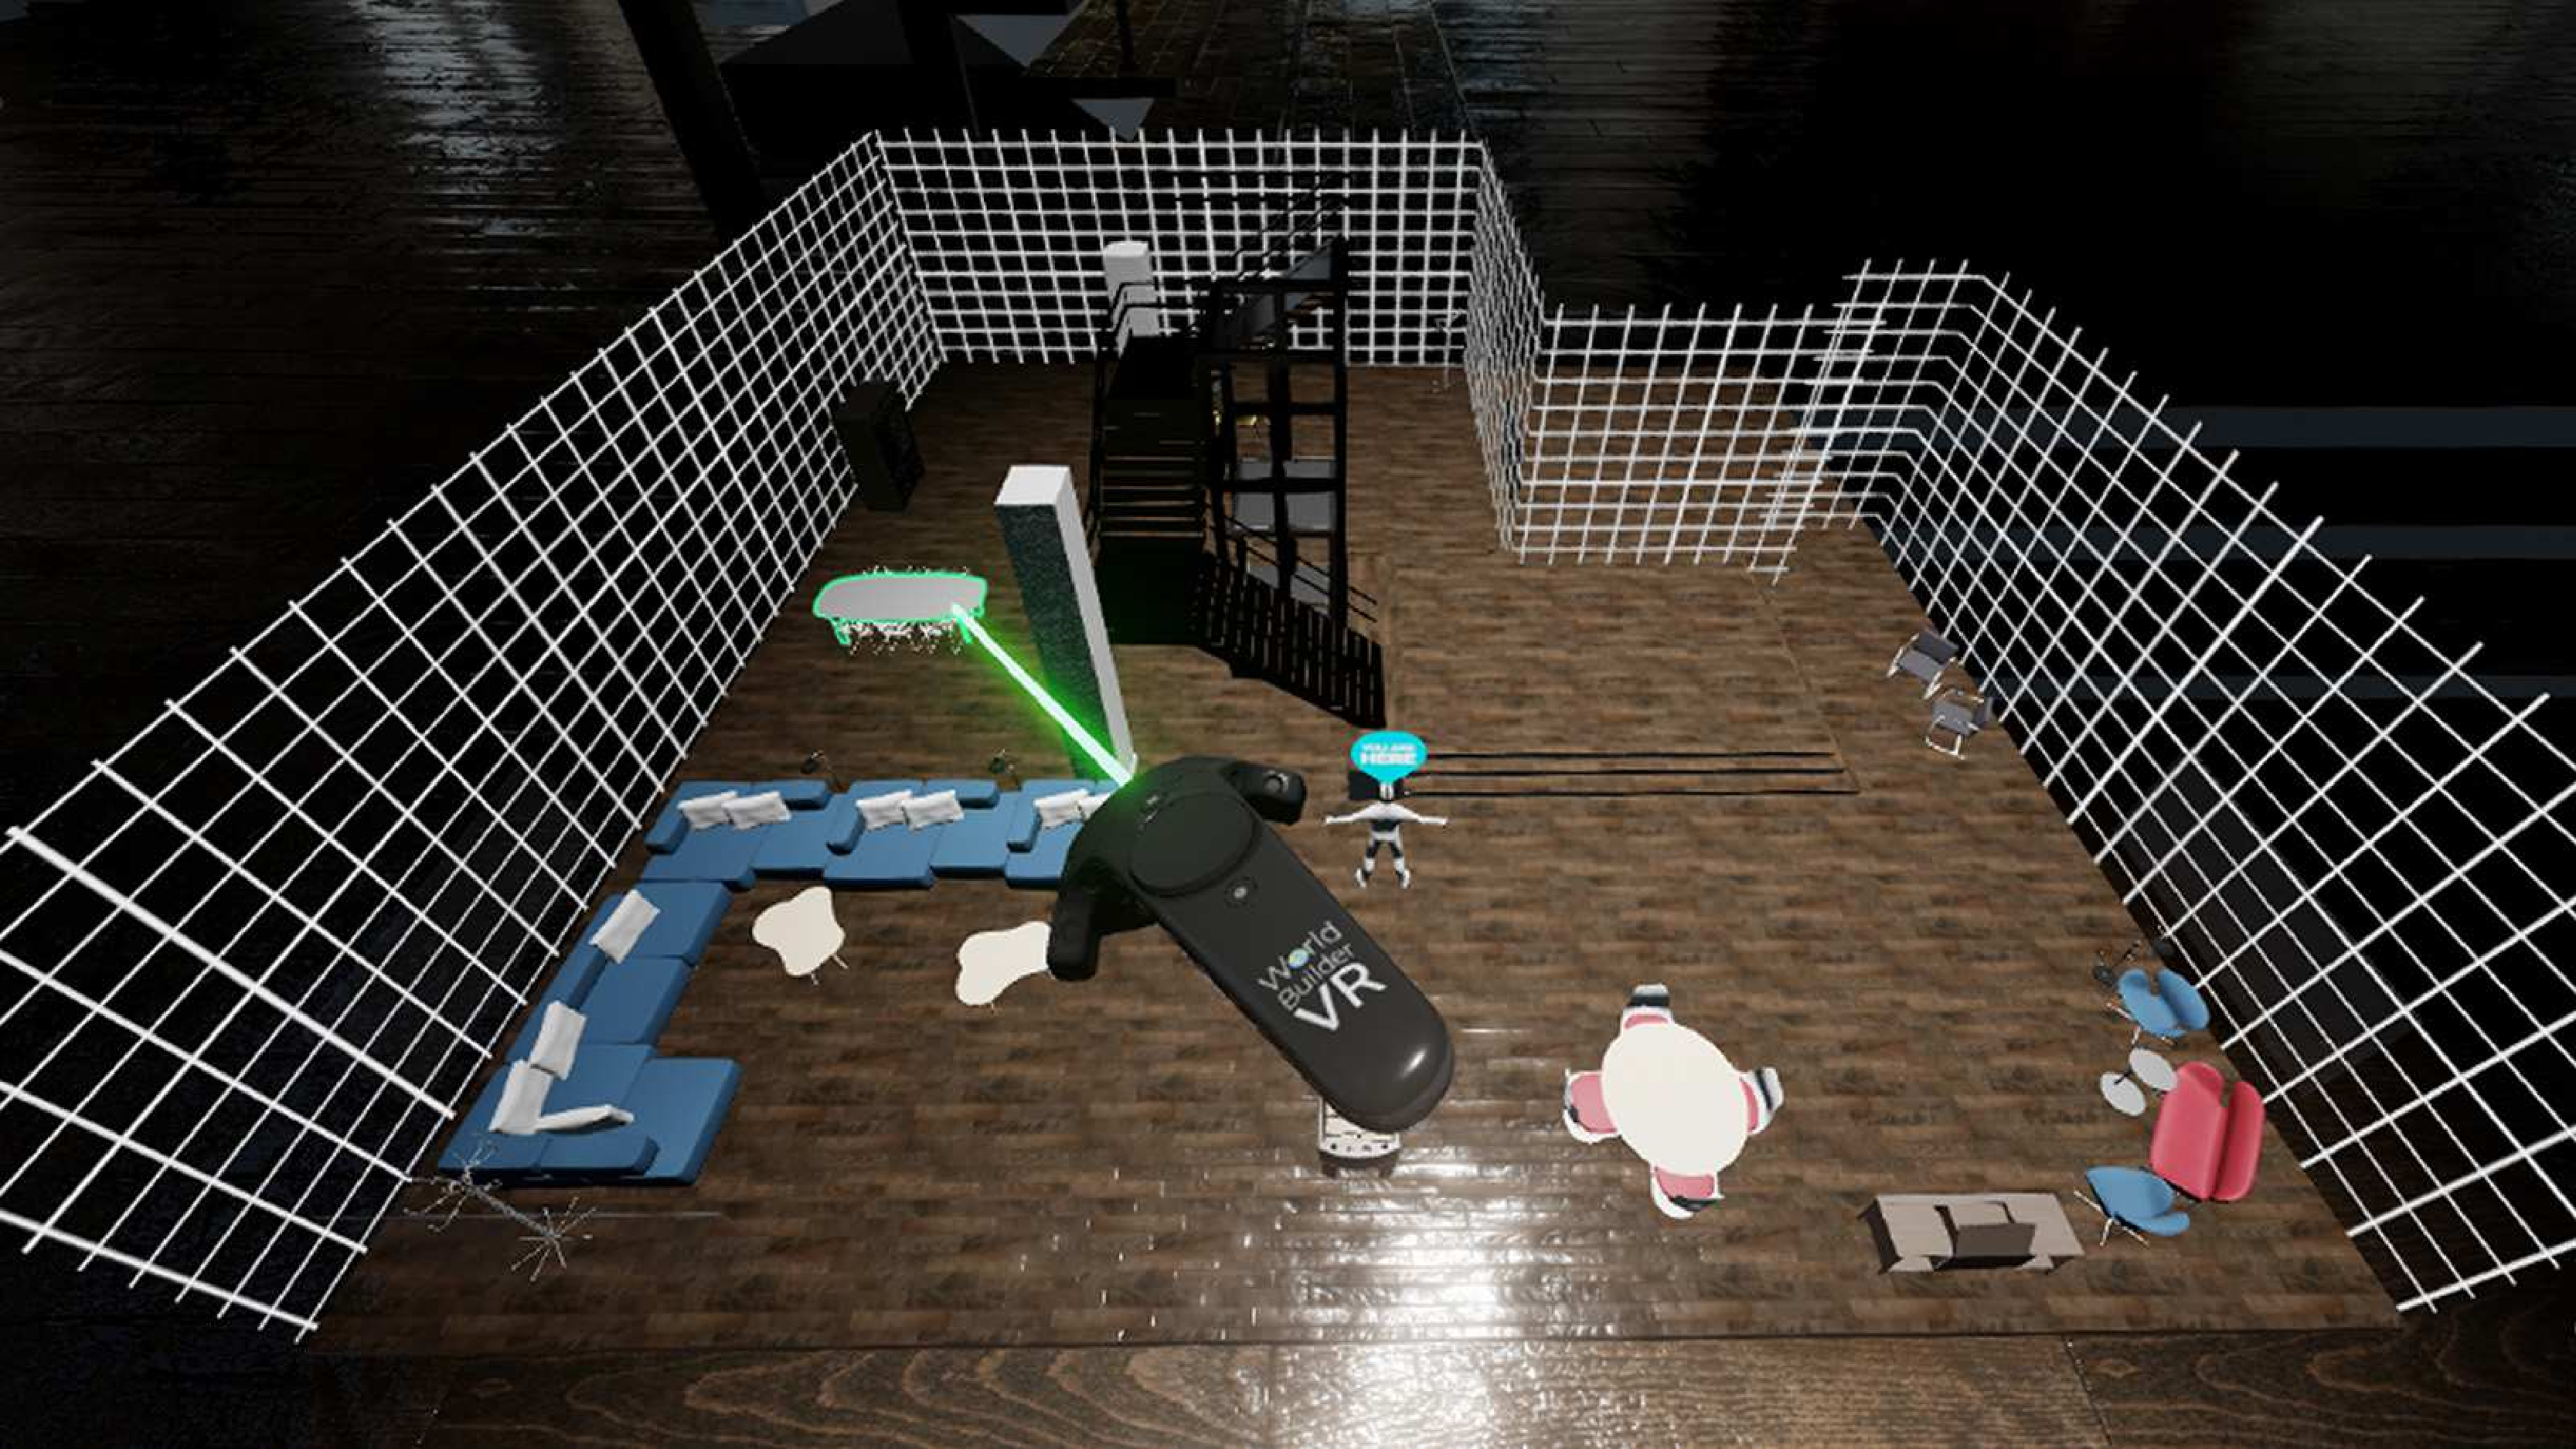
\includegraphics[width=14cm]{kapitel/eps/mini-map.pdf}
  \centering
  \caption{Mini map as part of the WIM technique. By \cite{Arnowitz.2017}}
  \label{fig:minimap}
\end{figure}
An alternative to this method is the \textbf{world in miniature (WIM) technique}. As seen in figure \ref{fig:minimap}, the user gets a miniature map of the virtual world with all selectable objects. The user can now select desired objects and see the selection in miniature map. With this method, the user looses their ego centred point of view. This can be seen as a decrease in an immerse experience, although it increases usability.

When it comes to moving in a virtual world, there is a conflict between limited space in the real world and the unlimited virtual world \cite{Sherman.2019}. It is possible to collide with real world objects while wearing a HMD. Therefore, we describe some techniques by \cite{Dorner.2013} on how to deal with the problems of navigating through virtual worlds:\\
One method of moving around in VR can be direct manipulation of the camera with a suitable input controller. For example, the user moves the camera with the help of a joystick. Another method which is very common in 3D computer games and therefore matches with the expectations of users, is walking in the direction of the user's point of view. A disadvantage of this method is that the user cannot look around while moving. Both described techniques have the disadvantage of possible motion sickness. This phenomenon will be described in chapter \ref{limits}.\\
In order to overcome the problem of motion sickness, teleporting is used instead, which is a very common technique for navigation. Teleporting means translating the user directly to a specific position without a time delay. This technique can be realised in VR by selecting the desired translation point via ray-casting and jumping to the point after selection. This method successfully handles the problem of motion sickness, but there is a loss of immersion, since this kind of navigation is not very natural.  \cite{Bozgeyikli.2016}\\
The most natural and immerse way of navigating is physical walking. Walking in a virtual environment deals with the above mentioned conflict between real and virtual world space. Natural walking in general needs more complex hardware for tracking the user's movement than navigation with the help of a controller. One method of walking in VR is the walking in place method. As the name describes, the user moves in the virtual world by lifting their legs but they are not actually changing their position in the real world. There are several hardware installations which support walking in place, some of them make walking possible through a treadmill system.\\
It is also possible to let the user walk around in a special room, that was designed for virtual reality usage and provides suitable tracking sensors. To avoid colliding with the real world borders of the room, the redirected walking technique was developed. With this technique it is possible to feign the user a straight path in the virtual world, while they are actually moving a different path to avoid walls. The difference between virtual and actual path are seen in figure \ref{fig:walking}.
\begin{figure}[h!]
  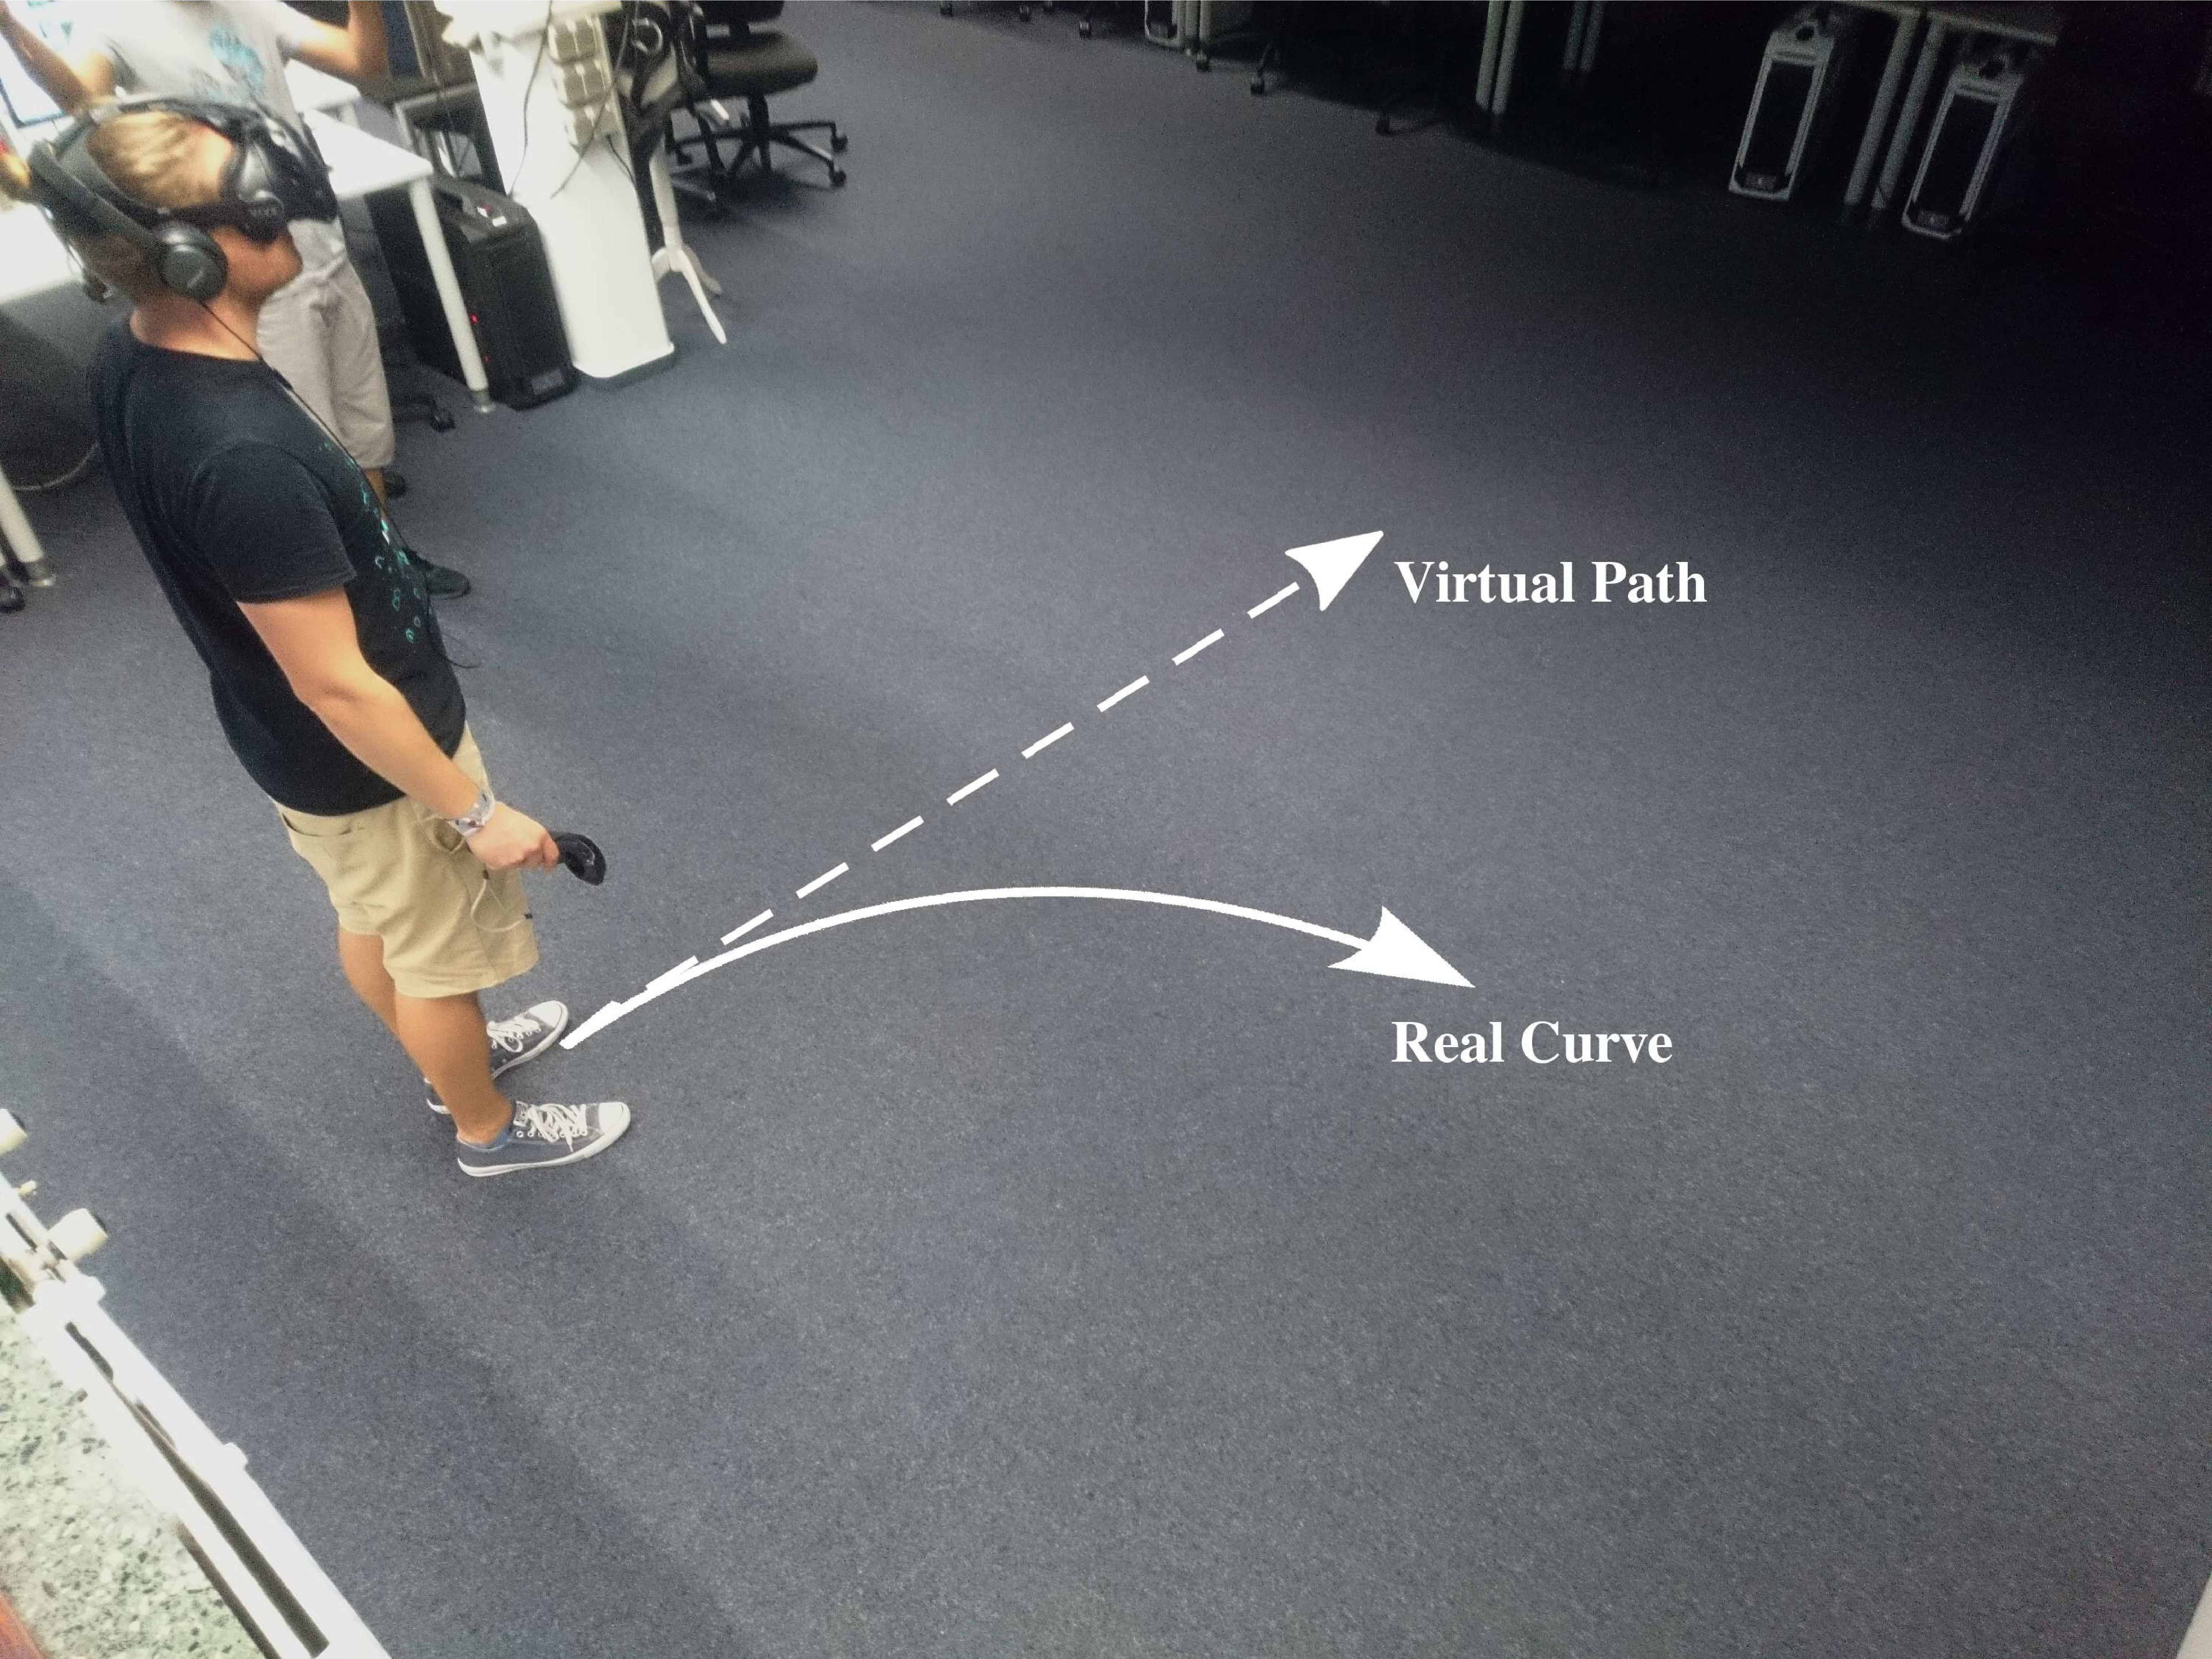
\includegraphics[width=10cm]{kapitel/eps/redirected-walking.pdf}
  \centering
  \caption{Redirected walking in VR, virtual walking path vs. actual walking path. By \cite{LS18}}
  \label{fig:walking}
\end{figure}

\section{Hardware for virtual reality} \label{hardware}
Some important objectives when it comes to new hardware technologies in VR are increase of immersion, reducing of costs and decreasing of size and weight. The two main types of HMDs currently available are desktop HMDs and mobile HMDs. The first type runs a game on a standalone desktop and the HMD measures the sensorical data from the user. The second type uses the phone to run a game and the phone's sensors to measure head rotation and other relevant data. In general, desktop HMDs have a stronger performance than the mobile HMDs because the game is processed on a standalone desktop PC instead of a phone inside the HMD. \cite{Dorner.2013}\\
An additional third type of HMDs are standalone devices. They are similar to mobile VR headsets but there is no need of attaching a mobile phone into the HMD. Instead, the device works out of the box. The performance of such standalone devices is lower than desktop dvices but higher than the mobile HMDs. \cite{Vitillo}\\
Current HMDs on the market can be divided into three categories: Low cost consumer HMDs, high end consumer HMDs for frequent VR players and high standard VR headsets, targeting customers in the industry. Looking at the new VR headset which are announced for 2019, the low cost VR headsets are improved in weight and screen resolution. Many of the new devices are mobile or standalone products, like the Oculus Quest. The high end VR headsets for private and industry customers introduce also the technique of eye-tracking, like the HTC Vive Pro Eye, and new display techniques. In general, there is more variety of VR headset products and manufacturers in the year 2019 in comparison to the previous years. \cite{Pertzborn.2019}\\
In this project, the application is deployed on two different devices which belong to the low cost category. The devices provided for development are Samsung Gear VR and Oculus Go. In the following, we compare the two devices and point out their advantages and disadvantages. Both devices can be seen in figure \ref{fig:devices}.

\begin{figure}[h!]
  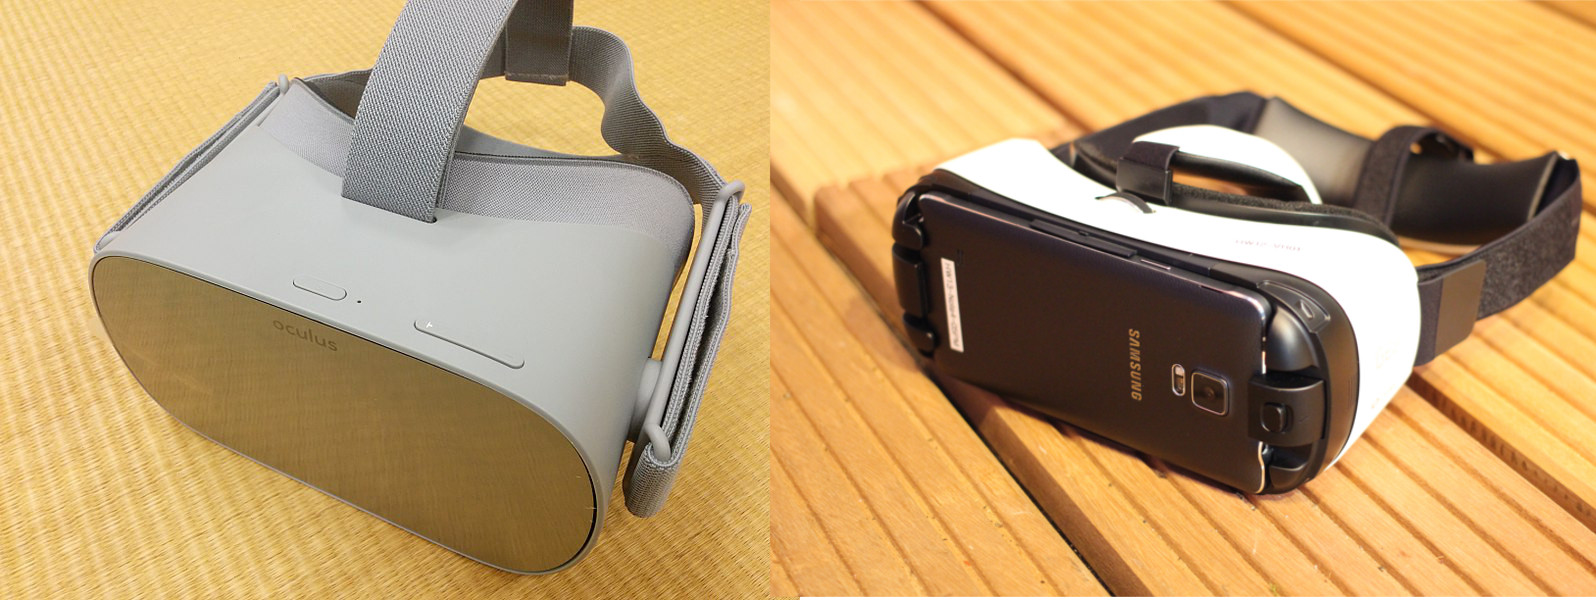
\includegraphics[width=13cm]{kapitel/oculus-samsung}
  \centering
  \caption{Oculus Go headset (left) by \cite{oculus} and Samsung Gear VR headset by \cite{hmd1}}
  \label{fig:devices}
\end{figure}
\newpage 
\paragraph{Samsung Gear VR} Samsung Gear VR is a mobile based VR headset, which was developed by Samsung and Oculus and introduced in 2017. The performance and screen resolution of the HMD depends on the mobile phone used with the headset. Gear VR is currently supported only by recent Samsung phones including Galaxy S6 and higher, Galaxy Note 5 and higher, Galaxy A8 and higher.
It comes with a bluetooth handheld controller which can either be held in the left or right hand. Embedded in the HMD there is a gyro sensor to detect head rotation. There is a proximity sensor as well inside the headset to detect if the user is currently wearing the HMD. The device does not support motion controlling, like walking. \cite{Samsung.2019}\\
Gear VR is supported by the game engine unity which makes the software application development easier. However, the use of a Samsung mobile phone is required, and not all Samsung phones are supported.
\paragraph{Oculus Go}
This device was announced in May 2018 and is a standalone device.
Inside the HMD is a Qualcomm Snapdragon processor which is widely used in smartphones. The screen resolution is  2560 x 1440 pixel. This resolution is comparable to high class smartphones of the year 2018 and therefore comparable to the Gear VR in combination with a suitable smartphone. The sensors and the handheld controller are very similar to the Samsung Gear VR device.\\
Looking at the technical data, there is not much of a difference between the two devices. Nevertheless, an advantage of the Oculus Go is that no phone has to be attached to the device. Also the head strap and the audio output were improved.\cite{Robertson.2018}
\section{Showcases of VR applications}
\label{labster}
There are a variety of VR applications available for very different use cases and made with different concepts. In this section we present the game \textit{Labster} which is an educational learning application and was ported to VR.\\
The objective of Labster is teaching university students new topics in biology and chemistry by self exploring and self-teaching instead of a frontal class. This objective is very similar to the goals of this work where we aim to let students explore IT job roles instead of getting only passive information. Labster has multiple scenarios that contain an interesting storyline. The stories are real life problems which can be solved by using the introduced knowledge about chemistry and biology, such as solving a murder case. Most of the time, the scenes take place in 3D laboratory where users can choose to work with different instruments and learn how to use them. A study from the founder of the product, , found out that students show better results in tests when they learned the topics with Labster instead of front teaching. \cite{Bodekaer.October2015} \\
We were not able to test the game, but from watching walkthrough videos and reviews, we tried to reconstruct, how Labster creates an immerse experience and is educational at the same time.
The first thing, that Labster focus on is a good storyline: It connects the theoretical knowledge with a real life scenario and in the same time introduces job fields in biology and chemistry. The students learn that they can do something meaningful with their knowledge which motivates them and let them immerse deeper with the game. Secondly, Labster guides users by having dialogues with an assistant and showing textual hints when hovering over interactive items. This helps that users do not feel disoriented and can focus on solving the tasks instead of figuring out how user interactions .\\
The game Labster can be seen as a good example and role model for the prototype application. In chapter \ref{design} we will discuss what concepts seen in Labster can be useful for the VR prototype in this work.
\section{Limits of virtual reality} \label{limits}
The idea of VR is not a new invention of the past few years. There has already been a peek in research and also prominence to the public in the late 90's and beginning of 2000. However, the technology did not prevail in the economy, because there were several limitations especially in performance of computation. Therefore only a limited amount of ideas were able to be actually implemented. Another problem at that time were the very large and heavy HMDs. The user could not wear them for a very long time and it caused neck pain and other physical problems. The devices were also not portable. \cite{Jerald.2016}\\
Looking at VR technologies now, a lot has changed. At first, the performance of our processors have increased rapidly. Secondly the HMDs became a lot smaller and lighter compared to the ones of the late 90's. But yet, we are not at the point, where all research is done -- on the contrary: A lot of challenges still occur when creating a VR application today. In the following, the problem of motion sickness is explained. We point out, what solutions are upcoming in the near future. There is also a lot of research in progress, when it comes to maximise physical immersion. We explained, what interactions cannot be covered by today's hardware, and what technologies are in development or testing at current stage.
\subsection{Motion sickness}
Motion sickness is a very common problem in VR. It can be compared to the kind of sickness some people experience when sitting in moving vehicles, such as buses, cars or roller coasters. The symptoms are nausea, dizziness or even vomit. Most of the time these symptoms occur after a usage time of more than ten minutes. Unfortunately, motion sickness does occur on a very large percentage of people and therefore cannot be ignored easily. In the study of \cite{Siess.2017}, over a half of the test persons experienced one of the described symptoms during playing a VR roller coaster game.\\
The most likely reason for motion sickness in VR is the mapping between real movement and virtual movement. For example, there is a high propability of feeling sick, when there is a latency between head movement and the movement in the virtual world. This latency  will be registered by the brain and is experienced as unfamiliar. Other situations, such as walking in the virtual world without physically moving can be a reason for motion sickness as well. \cite{Dorner.2013} \\ \cite{Siess.2017} also listed other reasons such as excessive speeds, for example first person moving speed or the moving speed of nearby obstacles, insufficient graphics or general technical problems( e.g. quality of lenses or comfort of HMD).
\cite{Fenlon.2013} mentions the removal of player control as a reason for motion sickness. It is more likely to experience the symptoms if the games takes control over the head rotation instead of the player. \\
To overcome the problem of motion sickness, the latency between physical and virtual movement has to be as small as possible. This is of course limited by the performance of the hardware devices. Many creators try to manage the problem by creating short time experiences with less than ten minutes durance and trying to avoid fast moving objects in their application. \cite{Doerner.2013}\\
This approach however, limits the possibilities in VR games. It would be hard to create an action shooter without fast moving objects, for example. \\
Besides this constraints, there have been new hardware developments lately which promise to solve the problem of motion sickness in VR. One of this hardware inventions is a device by \cite{Sra:2019} which stimulates the galvanic vestibular systems. User wear a necklace with electrodes placed behind the ear. Everytime users move in the virtual world, there is a electric stimulation of the vestibular system. According to \cite{Sra:2019} this should simulate a movement to the brain. The gap between physical and virtual movement can be tricked in a way through the device. However, the device is still a prototype and so far, it has been tested with only 20 participants. There have to be more clinical studies until a clear statement of the effectiveness can be made.\\
Looking at the VR prototype application which will be developed during this work the risk of motion sickness should be held to a minimum. To fulfil this requirement, there has to be a balance between a high level of immersion and the reducing of motion sickness. How this is realized we will describe in chapter \ref{design} and \ref{implementation}.

\subsection{Hardware}
There are several limitations in hardware devices when it comes to VR at the time of writing. First of all, the sensors of a HMD have to work very accurate. Also computation of the head movement and the virtual world movement has to be as fast as possible. The display resolution of VR devices has to be a lot higher compared to TV screens or desktop screens, because there is a magnification of the pixels through the lenses inside HMDs \\
When looking at physical immersion, there are a lot of potential enhancements in providing the user a more natural way of interacting with the virtual world. Most of the currently available HMDs for consumers require handheld controllers for user interaction. A body tracking system would provide more immersion, but requires very accurate sensors. The HTC Vive uses body positioning techniques but still needs handheld controllers.
Relocating the player in the virtual world is also a challenge at the time of writing. In chapter \ref{interaction-state-of-art} the usage of a treadmill system was already mentioned. The following section will present a current available VR treadmill for VR. Within this example the current limits of physical walking VR are explained.

In \cite{Cakmak.2014} the cyberith virtualizer is introduced. It is a device which supports natural walking in VR through the walking in place method. Users are wearing special shoes and lean into a belt system, which can be seen in figure TODO. The feet are sliding onto the surface and translated as a movement into the virtual world. The movement mapping is realized through various sensors which are placed into the ground floor of the treadmill. It is possible to use the cyberith virtualizer with controller specialized games, because the software of this treadmill is emulating controller input commands.\\
This device, however is not yet available on the consumer market. The company had problems of finding customers after announcing and presenting it in 2014. In 2016 they announced that they would concentrate on the B2B market. \cite{Skarredghost.2019}\\
The reasons for this could be the expensive price and also the large size of the device. The consumer market might not be ready yet for devices like that. This example shows how challenging it is for commercial companies to make innovations in VR. Therefore it is important to push public scientific research in VR further forward.

\section{Measurement of effectiveness of VR technologies}
Since we talked about new technologies and its limits in the previous section, the question is now how to measure the impact of VR technologies. How can we be sure that a new technology, hardware or software, actually fulfils the promises? Measurements like performance, screen resolution or weight are criteria which are easy to measure and compare. It is more difficult, to see how effective a VR technology is when it comes to user experience and immersion. In the prototype of this work, we focus on these measurements. \\
We focused our research in finding usability tests which deal with the topics of immersion, presence and user experience. The questionnaire from \cite{Witmer.1998} focus on immersion and presence and includes the factors of control, sensory, distraction and realism. This questionnaire can be very useful for usability tests on the VR prototype in this work. However, we could not find a questionnaire which measures the understanding of job roles or similar objectives. Therefore, a new questionnaire has to be developed for the user testing.